% Options for packages loaded elsewhere
\PassOptionsToPackage{unicode}{hyperref}
\PassOptionsToPackage{hyphens}{url}
%
\documentclass[
]{article}
\usepackage{amsmath,amssymb}
\usepackage{iftex}
\ifPDFTeX
  \usepackage[T1]{fontenc}
  \usepackage[utf8]{inputenc}
  \usepackage{textcomp} % provide euro and other symbols
\else % if luatex or xetex
  \usepackage{unicode-math} % this also loads fontspec
  \defaultfontfeatures{Scale=MatchLowercase}
  \defaultfontfeatures[\rmfamily]{Ligatures=TeX,Scale=1}
\fi
\usepackage{lmodern}
\ifPDFTeX\else
  % xetex/luatex font selection
\fi
% Use upquote if available, for straight quotes in verbatim environments
\IfFileExists{upquote.sty}{\usepackage{upquote}}{}
\IfFileExists{microtype.sty}{% use microtype if available
  \usepackage[]{microtype}
  \UseMicrotypeSet[protrusion]{basicmath} % disable protrusion for tt fonts
}{}
\makeatletter
\@ifundefined{KOMAClassName}{% if non-KOMA class
  \IfFileExists{parskip.sty}{%
    \usepackage{parskip}
  }{% else
    \setlength{\parindent}{0pt}
    \setlength{\parskip}{6pt plus 2pt minus 1pt}}
}{% if KOMA class
  \KOMAoptions{parskip=half}}
\makeatother
\usepackage{xcolor}
\usepackage[left=3cm,right=3cm,top=2cm,bottom=2cm]{geometry}
\usepackage{graphicx}
\makeatletter
\def\maxwidth{\ifdim\Gin@nat@width>\linewidth\linewidth\else\Gin@nat@width\fi}
\def\maxheight{\ifdim\Gin@nat@height>\textheight\textheight\else\Gin@nat@height\fi}
\makeatother
% Scale images if necessary, so that they will not overflow the page
% margins by default, and it is still possible to overwrite the defaults
% using explicit options in \includegraphics[width, height, ...]{}
\setkeys{Gin}{width=\maxwidth,height=\maxheight,keepaspectratio}
% Set default figure placement to htbp
\makeatletter
\def\fps@figure{htbp}
\makeatother
\setlength{\emergencystretch}{3em} % prevent overfull lines
\providecommand{\tightlist}{%
  \setlength{\itemsep}{0pt}\setlength{\parskip}{0pt}}
\setcounter{secnumdepth}{-\maxdimen} % remove section numbering
\usepackage{float}
\ifLuaTeX
  \usepackage{selnolig}  % disable illegal ligatures
\fi
\IfFileExists{bookmark.sty}{\usepackage{bookmark}}{\usepackage{hyperref}}
\IfFileExists{xurl.sty}{\usepackage{xurl}}{} % add URL line breaks if available
\urlstyle{same}
\hypersetup{
  hidelinks,
  pdfcreator={LaTeX via pandoc}}

\author{}
\date{\vspace{-2.5em}}

\begin{document}

\begin{titlepage}
\centering
\vspace*{5cm}
{\Large\bfseries PSTAT 172A Project:\\[0.5em]
Pricing Insurance and Setting a Security Loading\par}
\vspace{2cm}
{\large Author: Zejie (Sandy) Gao\par}
{\large University of California, Santa Barbara\par}
{\large PSTAT 172A: Actuarial Statistics I\par}
{\large Instructor: Dr. Hal Pedersen\par}
{\large Winter 2024\par}
\vspace*{\fill}
\end{titlepage}

\newpage

\emph{Background}

You are the pricing actuary for your insurance company. You are asked to
analyze a whole life insurance policy on (60) for which the benefit of
\$1,000 is paid at the end of the year of death. Assume that the
effective annual interest rate is 6\% (i.e., i=0.06).

\hypertarget{compute-the-net-single-premium-for-the-policy.}{%
\section{1. Compute the net single premium for the
policy.}\label{compute-the-net-single-premium-for-the-policy.}}

Under the equivalence principle, the premium is set such that the
expected value of the loss for the random variable at issue is zero. The
equation for the net single premium will be as follows:

\begin{center}
  \textbf{EPV of premium income = EPV of benefit outgo}
\end{center}

Here is the head of the modified data set:

\begin{verbatim}
## # A tibble: 6 x 7
##       x     qx     k discount_factor    px   kpx sqr_discount_factor
##   <dbl>  <dbl> <int>           <dbl> <dbl> <dbl>               <dbl>
## 1    60 0.0135     0           0.943 0.987 1                   0.890
## 2    61 0.0146     1           0.890 0.985 0.987               0.792
## 3    62 0.0157     2           0.840 0.984 0.972               0.705
## 4    63 0.0168     3           0.792 0.983 0.957               0.627
## 5    64 0.0179     4           0.747 0.982 0.941               0.558
## 6    65 0.0189     5           0.705 0.981 0.924               0.497
\end{verbatim}

The next step is to sum over all possible payment times, taking the
product of the benefit amount, the corresponding discount factors, and
the probability that the benefit will be paid at that time.
Alternatively, this can be expressed as the benefit amount multiplied by
\(A_{60}\).

\begin{verbatim}
## Whole life insurance at Age 60: $ 0.3455611
\end{verbatim}

\begin{verbatim}
## Benefit Amount: $ 1000
\end{verbatim}

\begin{verbatim}
## Expected Present Value of Benefit Outgo: $ 345.5611
\end{verbatim}

Thus, the net single premium for the policy is \$345.56, equivalent to
the expected present value of benefit outgo according to the equivalence
principle.

\hypertarget{compute-the-net-annual-premium-for-the-policy.}{%
\section{2. Compute the net annual premium for the
policy.}\label{compute-the-net-annual-premium-for-the-policy.}}

Under the equivalence principle, we can drive the annual premium as the
equation:

\[
B * A_{60} = P_{60}*\ddot{a}_{{60}}
\]

\begin{verbatim}
## Whole life annuity-due at Age 60: $ 11.56175
\end{verbatim}

\begin{verbatim}
## Net annual premium:$ 29.8883
\end{verbatim}

Thus, the net annual premium for the policy is \$29.89.

\hypertarget{determine-the-single-premium-for-the-policy-for-a-group-of-2500-identical-insureds-so-that-the-probability-of-a-loss-is-less-than-or-equal-to-0.025.}{%
\section{3. Determine the single premium for the policy for a group of
2,500 identical insureds so that the probability of a loss is less than
or equal to
0.025.}\label{determine-the-single-premium-for-the-policy-for-a-group-of-2500-identical-insureds-so-that-the-probability-of-a-loss-is-less-than-or-equal-to-0.025.}}

Let's denote \(P^{\epsilon}\) as the single premium for the policy.
Then, the loss for individual policy will be

\(L^{(i)} = 1000*v^{k^{(i)}_x+1}-P^{\epsilon}\).\\
By using CLT, we can approximate the sum of the 2,500 identical
insured's Loss \(L\) minus mean \(\mu = N*E[L^{(i)}]\) divided by
\(\sigma = (N* Var[L^{(i)}])^{0.5}\) follows a standard normal
distribution.

\begin{itemize}
\item
  \(E[L^{(i)}]\) is the EPV of Benefit outgo minus \(P^{\epsilon}\) ,
  which is \(1000*A_{60} - P^{\epsilon}\)
\item
  \(Var[L^{(i)}])\) = \(1000^2*\sigma^2_{A_{60}}\)
\item
  \(N = 2500\)
\end{itemize}

So \(P(L > 0 ) = 0.025\) is equivalent to
\(P(Z > \frac{0-\mu}{\sigma}) = 0.025\), that is to say find out the
\(P^{\epsilon}\) to satisfy: \[
\Phi(\frac{-\mu}{\sigma}) = 0.975
\]

\[
\frac{-N*(A_{60}-P^{\epsilon})}{(N* 1000^2*\sigma^2_{A_{60}})^{0.5}} = \zeta_{0.975}
\]

\[
\frac{(N)^{0.5}*(P^{\epsilon}-A_{60})}{1000*\sigma_{A_{60}}} = \zeta_{0.975}
\]

\[
P^{\epsilon} = \frac{1000}{(N)^{0.5}}*\zeta_{0.975}*\sigma_{A_{60}} + 1000*A_{60}
\]

\begin{itemize}
\item
  \(\sigma_{A_{60}} = 0.2042844\)
\item
  \(\zeta_{0.975} = 1.959964\)
\item
  \(A_{60} = 0.3455611\)
\end{itemize}

\begin{verbatim}
## Single premium for this policy under problem 3's condition is $ 353.5689
\end{verbatim}

Thus, the single premium for the policy for a group of \(2,500\)
identical insureds so that the probability of a loss is less than or
equal to 0.025 is \$353.57.

\hypertarget{determine-the-annual-premium-for-the-policy-for-a-group-of-2500-identical-insureds-so-that-the-probability-of-a-loss-is-less-than-or-equal-to-0.025.}{%
\section{4. Determine the annual premium for the policy for a group of
2,500 identical insureds so that the probability of a loss is less than
or equal to
0.025.}\label{determine-the-annual-premium-for-the-policy-for-a-group-of-2500-identical-insureds-so-that-the-probability-of-a-loss-is-less-than-or-equal-to-0.025.}}

Let's denote \(P^{\epsilon}\) as the annual premium for the policy.
Then, the loss for individual policy will be

\[
L^{(i)} = 1000*v^{k^{(i)}_x+1}-P^{\epsilon}_x*\ddot{a}_{k^{(i)}_x+1}.
\]

By using CLT, we can approximate the sum of the 2,500 identical
insured's Loss \(L\) minus mean \(\mu = N*E[L^{(i)}]\) divided by
\(\sigma = (N* Var[L^{(i)}])^{0.5}\) follows a standard normal
distribution.

\begin{itemize}
\item
  \(E[L^{(i)}]\) is the EPV of Benefit outgo minus EPV of income, which
  is \(1000*A_{60} - P^{\epsilon}_{60}*\ddot{a}_{60}\).
\item
  \(A_{60} = P_{60}*\ddot{a}_{60}\), where \(P_{60}\) is the net annual
  premium.
\item
  \(Var[L^{(i)}])\) =
  \(\left(1000+\frac{P_x^{\varepsilon}}{d}\right)^2 \sigma^2_{A_{60}}\)
\item
  \(N = 2500\)
\end{itemize}

So, \(P(L > 0 ) = 0.025\) is equivalent to
\(P(Z > \frac{0-\mu}{\sigma}) = 0.025\), that is to say find out the
\(P^{\epsilon}\) to satisfy:

\[
\Phi(\frac{-\mu}{\sigma}) = 0.975
\]

\[
\frac{N*(P^{\epsilon}_{60}-P_{60})*\ddot{a}_{60}}{N^{0.5}* \left(1000+\frac{P_{60}^{\varepsilon}}{d}\right) \sigma_{A_{60}}} = \zeta_{0.975}
\]

\[
\frac{N^{0.5}*(P^{\epsilon}_{60}-P_{60})*\ddot{a}_{60}}{ \left(1000+\frac{P_{60}^{\varepsilon}}{d}\right) \sigma_{A_{60}}} = \zeta_{0.975}
\]

\[
(P^{\varepsilon}_{60} - P_{60})\ddot{a}_{60} = \frac{\zeta_{0.975} \sigma_{A_{60}}}{\sqrt{N}} 1000 + \frac{\zeta_{0.975} \sigma_{A_{60}}}{\sqrt{N}} \cdot \frac{P^{\varepsilon}_{60}}{d}
\]

\[
P^{\varepsilon}_{60}\ddot{a}_{60} - \frac{\zeta_{0.975} \sigma_{A_{60}}}{d\sqrt{N}} P^{\varepsilon}_{60} = P_{60}\ddot{a}_{60} + \frac{\zeta_{0.975} \sigma_{A_{60}} 1000}{\sqrt{N}}
\]

\[
P^{\varepsilon}_{60} \left(\ddot{a}_{60} - \frac{\zeta_{0.975} \sigma_{A_{60}}}{d\sqrt{N}}\right) = P_{60}\ddot{a}_{60} + \frac{\zeta_{0.975} \sigma_{A_{60}} 1000}{\sqrt{N}}
\]

\[
P^{\varepsilon}_{60} = \frac{P_{60}\ddot{a}_{60} + \frac{\zeta_{0.975} \sigma_{A_{60}} 1000}{\sqrt{N}}}{\ddot{a}_{60} - \frac{\zeta_{0.975} \sigma_{A_{60}}}{d\sqrt{N}}}
\]

\[
P^{\epsilon}_{60} = \frac{P_{60} + 1000*\frac{\zeta_{0.975}*\sigma_{A_{60}}}{(N)^{0.5}*\ddot{a}_{{20}}}}{1-\frac{\zeta_{0.975}*\sigma_{A_{60}}}{(N)^{0.5}*\ddot{a}_{{20}}*d}}
\]

\begin{itemize}
\item
  \(N = 2500\)
\item
  \(d = \frac{i}{1+i}\)
\item
  \(P_{60}\) is calculated form problem 2 which is \$29.88.
\end{itemize}

\begin{verbatim}
## Annual premium for this policy under problem 4's condition is $ 30.95974
\end{verbatim}

Thus, the annual premium for the policy for a group of \(2,500\)
identical insureds so that the probability of a loss is less than or
equal to 0.025 is \$30.96.

\hypertarget{what-happens-to-the-single-and-annual-premiums-as-the-number-of-identical-insureds-increases-under-the-premium-calculations-in-3-and-4}{%
\section{5. What happens to the single and annual premiums as the number
of identical insureds increases under the premium calculations in 3 and
4?}\label{what-happens-to-the-single-and-annual-premiums-as-the-number-of-identical-insureds-increases-under-the-premium-calculations-in-3-and-4}}

From the equation in 3:

\[
P^{\epsilon}_x= \frac{1000}{(N)^{0.5}}*\zeta_{0.975}*\sigma_{A_{60}} + 1000*A_{60}
\]

From this equation, as \(N \to \infty\), the first term involving
\(\zeta_{0.975}\)and \(\sigma_{A_{60}}\) will approaches zero.
Therefore, as N grows very large, the single premium \(P^{\epsilon}_x\)
for this policy under these conditions approaches \(1000*A_{60}\), or
\$345.56.

From the equation in 4:

\[
P^{\epsilon}_{60} = \frac{P_{60} + 1000*\frac{\zeta_{0.975}*\sigma_{A_{60}}}{(N)^{0.5}*\ddot{a}_{{20}}}}{1-\frac{\zeta_{0.975}*\sigma_{A_{60}}}{(N)^{0.5}*\ddot{a}_{{20}}*d}}
\]

From this equation, as \(N \to \infty\), annual premium P for this
policy under these conditions approaches \(P_{60}\), or \$29.88.

\hypertarget{produce-a-chart-of-the-single-and-annual-premiums-as-a-function-of-the-number-of-insureds-under-the-requirements-of-items-3-and-4-respectively.}{%
\section{6. Produce a chart of the single and annual premiums as a
function of the number of insureds under the requirements of items 3 and
4
respectively.}\label{produce-a-chart-of-the-single-and-annual-premiums-as-a-function-of-the-number-of-insureds-under-the-requirements-of-items-3-and-4-respectively.}}

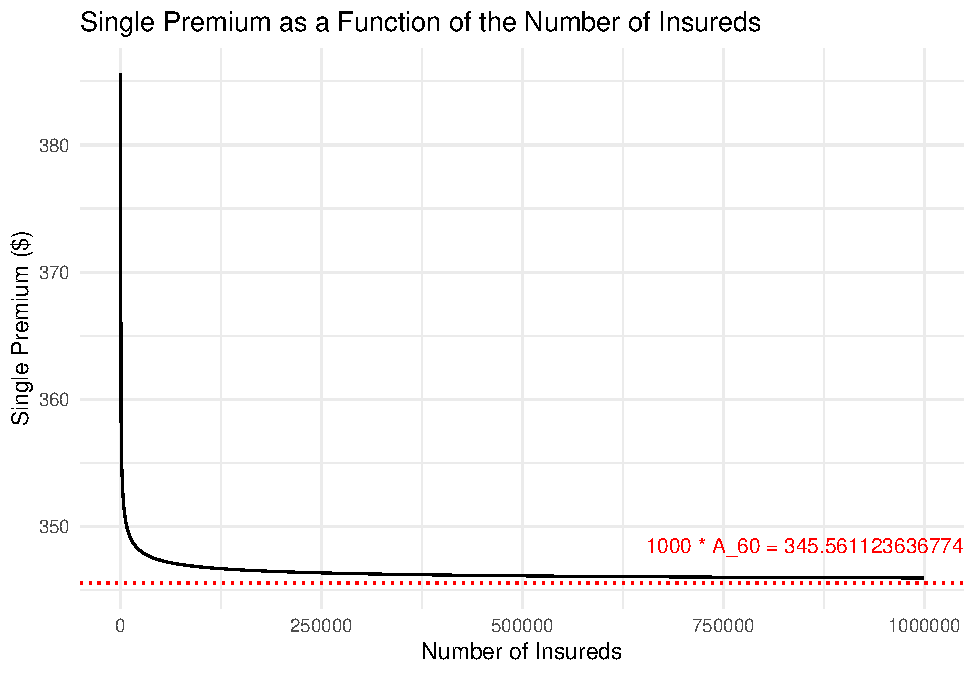
\includegraphics{Zejie--Sandy--Gao-172A-final-project_files/figure-latex/unnamed-chunk-10-1.pdf}

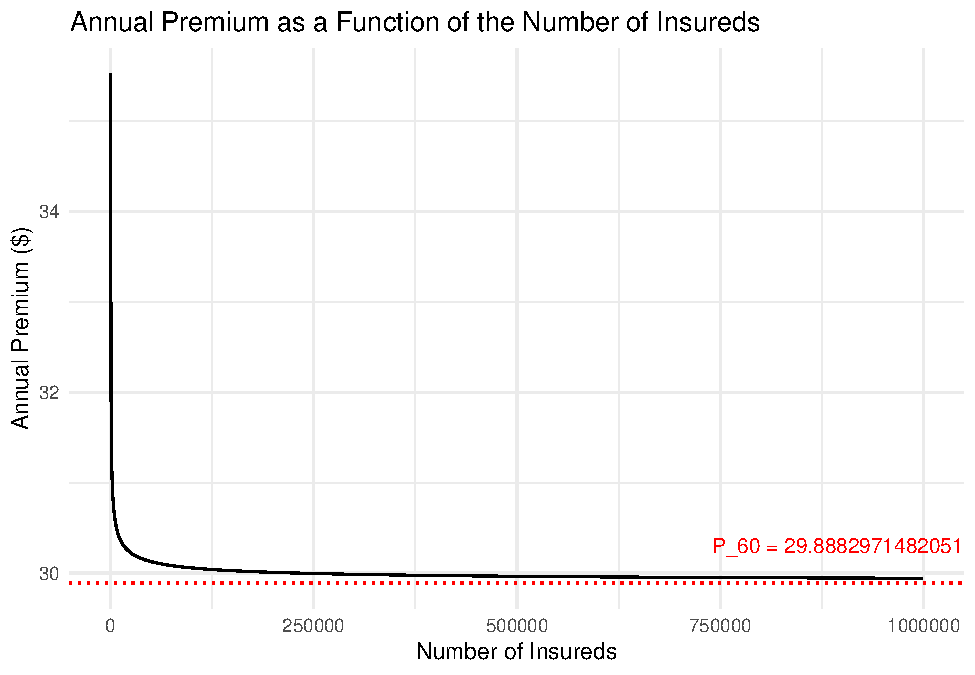
\includegraphics{Zejie--Sandy--Gao-172A-final-project_files/figure-latex/unnamed-chunk-11-1.pdf}

\hypertarget{now-assume-that-10-years-have-passed-and-there-are-2050-lives-remaining-from-the-original-pool-of-insureds.-how-much-reserve-should-the-insurer-have-per-policy-in-order-to-have-a-98-probability-of-not-losing-money-do-this-calculation-for-the-annual-premium-case.}{%
\section{7. Now assume that 10 years have passed and there are 2,050
lives remaining from the original pool of insureds. How much reserve
should the insurer have per policy in order to have a 98\% probability
of not losing money? Do this calculation for the annual premium
case.}\label{now-assume-that-10-years-have-passed-and-there-are-2050-lives-remaining-from-the-original-pool-of-insureds.-how-much-reserve-should-the-insurer-have-per-policy-in-order-to-have-a-98-probability-of-not-losing-money-do-this-calculation-for-the-annual-premium-case.}}

After 10 years each policy now has loss:

\[
L_{x, n}^{(i)}=1000*v^{k^{(i)}_{x+n}+1}-P_x^{\varepsilon} \ddot{a} _{k^{(i)}_{x+n}+1}.
\]

The Expected value of loss and the variance of loss per policy will be:

\[
\begin{aligned}
& \mathbb{E}\left[L_{x, n}^{(1)}\right]=1000*A_{x+n}-P_x^{\varepsilon} \ddot{a}_{x+n}, \\
& \operatorname{Var}\left[L_{x, n}^{(i)}\right]=\left(1000+\frac{P_x^{\varepsilon}}{d}\right)^2\left({}^2A_{x+n}-A_{x+n}^2\right).
\end{aligned}
\] The sum of loss for alive policyholder \(L_{x,n}\) and the reserve
per policy after n years \(R_n\) will have equations below:

\[
\begin{aligned}
& L_{x, n}=L_{x, n}^{(1)}+\cdots+L_{x, n}^{(m)} \text{, where } m=2,050. \\
& 0.02=P\left(L_{x, n}>R_n \cdot m\right). \\
& 0.02=P\left(\frac{L_{x, n}-\mathbb{E}\left[L_{x, n}\right]}{\sqrt{\operatorname{Var}\left(L_{x, n}\right)}}>\frac{R_n \cdot m-m\left[1000*A_{x+n}-P_x^{\varepsilon} \ddot{a}_{x+n}\right]}{\sqrt{m}\left(1000+\frac{P_{x}^{\varepsilon}}{d}\right) \sigma_{A_{x+n}}}\right). \\
& 0.02=1-\Phi\left(\frac{\sqrt{m}\left(R_n-\left[1000*A_{x+n}-P_x^{\varepsilon} \ddot{a}_{x+n}\right]\right)}{\left(1000+\frac{P_x^{\varepsilon}}{d}\right) \sigma_{A_{x+n}}}\right). \\
& \zeta_{0.98} =\left(\frac{\sqrt{m}\left(R_n-\left[1000*A_{x+n}-P_x^{\varepsilon} \ddot{a}_{x+n}\right]\right)}{\left(1000+\frac{P_x^{\varepsilon}}{d}\right) \sigma_{A_{x+n}}}\right). \\
& R_n=\left(\zeta_{0.98}\left(1000+\frac{P_x^{\varepsilon}}{d}\right) \sigma_{A_{x+n}}\right) \frac{1}{\sqrt{m}}+\left[1000*A_{x+n}-P_x^{\varepsilon} \ddot{a}_{x+n}\right], \quad\{x=60, n=10\}.
\end{aligned} 
\]

\[
R_{10}=\left(\zeta_{0.98}\left(1000+\frac{P_{60}^{\varepsilon}}{d}\right) \sigma_{A_{70}}\right) \frac{1}{\sqrt{2050}}+\left[1000*A_{70}-P_{60}^{\varepsilon} \ddot{a}_{70}\right].
\]

Given:

\begin{itemize}
\item
  The annual premium \(P_{60}^{\varepsilon}\) for a group of 2,500
  identical insured individuals aged 60 was calculated to ensure a loss
  probability of no more than 2.5\%, resulting in a premium of
  \$30.95974.
\item
  The same calculation method was applied to a dataset concerning
  mortality rates for individuals aged over 70, allowing for the
  estimation of actuarial values for this age group.
\end{itemize}

\begin{verbatim}
## $A_70
## [1] 0.4802804
## 
## $a_70_due
## [1] 9.181712
## 
## $sigma_A_70
## [1] 0.1992951
## 
## $zeta_0_98
## [1] 2.053749
## 
## $d
## [1] 0.05660377
\end{verbatim}

\begin{verbatim}
## Reserve Per Policy After 10 Years is: $ 210.0015
\end{verbatim}

Therefore, in order to have a 98\% probability of not losing money,
insuer should have reserve value \$ 210.00 per policy.

\hypertarget{discuss-the-benefit-and-drawbacks-of-charging-a-portfolio-level-premium-versus-a-net-premium-based-on-the-equivalence-principle.}{%
\section{8. Discuss the benefit and drawbacks of charging a portfolio
level premium versus a net premium based on the equivalence
principle.}\label{discuss-the-benefit-and-drawbacks-of-charging-a-portfolio-level-premium-versus-a-net-premium-based-on-the-equivalence-principle.}}

The Equivalence Principle and the Portfolio Percentage Premium Principle
(PPPP) provide distinct methods for calculating premiums for a policy.
Unlike the Equivalence Principle which determines premiums based on an
individual's expected loss, PPPP determines premiums based on the
expected loss of a large portfolio of identical and independent
policies.

Compared with the Equivalence Principle, there are several benefits for
PPPP. PPPP sets a level of premiums for all policyholders in the
portfolio, enhancing underwriting efficiency by saving time to determine
premiums separately. Also, it diverse the risk for the policyholders.
The third one is that it aids in stabilizing the financial outcomes for
insurance companies.

Moreover, PPPP is designed to achieve specific probabilistic objectives,
ensuring the probability of not losing money. While it controls the
probability of incurring a loss, it does not necessarily address the
size issue of the loss. This could pose a major problem if the loss is
significant enough to bankrupt the insurance company.

Therefore, although PPPP offers an efficient way to handle a large
number of policies, it requires careful management to mitigate the risk
of unexpected large losses.

\end{document}
